\documentclass{standalone}%
\usepackage[T1]{fontenc}%
\usepackage[utf8]{inputenc}%
\usepackage{lmodern}%
\usepackage{textcomp}%
\usepackage{lastpage}%
\usepackage{tikz}%
%
%
%
\begin{document}%
\normalsize%
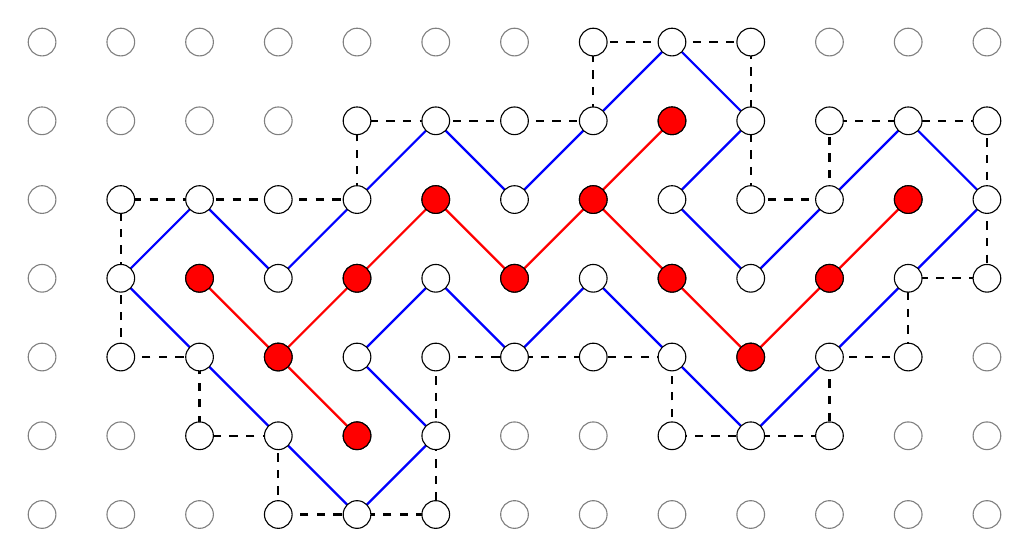
\begin{tikzpicture}[scale=1.0]%
\draw[thick, red] (6.0,-3.0) -- (5,-2)--(4,-3)--(3,-4)--(2,-3);
\draw[thick, red] (8.0,-1.0) -- (7.0,-2.0) -- (6.0,-3.0);
\draw[thick, red] (7.0,-2.0) -- (8,-3)--(9,-4)--(10,-3)--(11,-2);
\draw[thick, red] (3,-4)--(4,-5);
\draw[thick, blue] (8,0)--(9,-1)--(8,-2)--(9,-3)--(10,-2)--(11,-1)--(12,-2)--(11,-3)--(10,-4)--(9,-5)--(8,-4)--(7,-3)--(6,-4)--(5,-3)--(4,-4)--(5,-5)--(4,-6)--(3,-5)--(2,-4)--(1,-3)--(2,-2)--(3,-3)--(4,-2)--(5,-1)--(6,-2)--(7,-1)--(8,0);
\draw[thick, dashed] (7,0)--(9,0)--(9,-2)--(10,-2)--(10,-1)--(12,-1)--(12,-3)--(11,-3)--(11,-4)--(10,-4)--(10,-5)--(8,-5)--(8,-4)--(5,-4)--(5,-6)--(3,-6)--(3,-5)--(2,-5)--(2,-4)--(1,-4)--(1,-2)--(4,-2)--(4,-1)--(7,-1)--cycle;
\path[draw,radius=5pt, gray] (0.0,0.0) circle;%
\path[draw,radius=5pt, gray] (1.0,0.0) circle;%
\path[draw,radius=5pt, gray] (2.0,0.0) circle;%
\path[draw,radius=5pt, gray] (3.0,0.0) circle;%
\path[draw,radius=5pt, gray] (4.0,0.0) circle;%
\path[draw,radius=5pt, gray] (5.0,0.0) circle;%
\path[draw,radius=5pt, gray] (6.0,0.0) circle;%
\path[draw,radius=5pt, fill=white] (7.0,0.0) circle;%
\path[draw,radius=5pt, fill=white] (8.0,0.0) circle;%
\path[draw,radius=5pt, fill=white] (9.0,0.0) circle;%
\path[draw,radius=5pt, gray] (10.0,0.0) circle;%
\path[draw,radius=5pt, gray] (11.0,0.0) circle;%
\path[draw,radius=5pt, gray] (12.0,0.0) circle;%
\path[draw,radius=5pt, gray] (0.0,-1.0) circle;%
\path[draw,radius=5pt, gray] (1.0,-1.0) circle;%
\path[draw,radius=5pt, gray] (2.0,-1.0) circle;%
\path[draw,radius=5pt, gray] (3.0,-1.0) circle;%
\path[draw,radius=5pt, fill=white] (4.0,-1.0) circle;%
\path[draw,radius=5pt, fill=white] (5.0,-1.0) circle;%
\path[draw,radius=5pt, fill=white] (6.0,-1.0) circle;%
\path[draw,radius=5pt, fill=white] (7.0,-1.0) circle;%
\path[draw,radius=5pt, fill=white] (8.0,-1.0) circle;%
\path[draw,radius=5pt, fill=white] (9.0,-1.0) circle;%
\path[draw,radius=5pt, fill=white] (10.0,-1.0) circle;%
\path[draw,radius=5pt, fill=white] (11.0,-1.0) circle;%
\path[draw,radius=5pt, fill=white] (12.0,-1.0) circle;%
\path[draw,radius=5pt, gray] (0.0,-2.0) circle;%
\path[draw,radius=5pt, fill=white] (1.0,-2.0) circle;%
\path[draw,radius=5pt, fill=white] (2.0,-2.0) circle;%
\path[draw,radius=5pt, fill=white] (3.0,-2.0) circle;%
\path[draw,radius=5pt, fill=white] (4.0,-2.0) circle;%
\path[draw,radius=5pt, fill=white] (5.0,-2.0) circle;%
\path[draw,radius=5pt, fill=white] (6.0,-2.0) circle;%
\path[draw,radius=5pt, fill=white] (7.0,-2.0) circle;%
\path[draw,radius=5pt, fill=white] (8.0,-2.0) circle;%
\path[draw,radius=5pt, fill=white] (9.0,-2.0) circle;%
\path[draw,radius=5pt, fill=white] (10.0,-2.0) circle;%
\path[draw,radius=5pt, fill=white] (11.0,-2.0) circle;%
\path[draw,radius=5pt, fill=white] (12.0,-2.0) circle;%
\path[draw,radius=5pt, gray] (0.0,-3.0) circle;%
\path[draw,radius=5pt, fill=white] (1.0,-3.0) circle;%
\path[draw,radius=5pt, fill=white] (2.0,-3.0) circle;%
\path[draw,radius=5pt, fill=white] (3.0,-3.0) circle;%
\path[draw,radius=5pt, fill=white] (4.0,-3.0) circle;%
\path[draw,radius=5pt, fill=white] (5.0,-3.0) circle;%
\path[draw,radius=5pt, fill=white] (6.0,-3.0) circle;%
\path[draw,radius=5pt, fill=white] (7.0,-3.0) circle;%
\path[draw,radius=5pt, fill=white] (8.0,-3.0) circle;%
\path[draw,radius=5pt, fill=white] (9.0,-3.0) circle;%
\path[draw,radius=5pt, fill=white] (10.0,-3.0) circle;%
\path[draw,radius=5pt, fill=white] (11.0,-3.0) circle;%
\path[draw,radius=5pt, fill=white] (12.0,-3.0) circle;%
\path[draw,radius=5pt, gray] (0.0,-4.0) circle;%
\path[draw,radius=5pt, fill=white] (1.0,-4.0) circle;%
\path[draw,radius=5pt, fill=white] (2.0,-4.0) circle;%
\path[draw,radius=5pt, fill=white] (3.0,-4.0) circle;%
\path[draw,radius=5pt, fill=white] (4.0,-4.0) circle;%
\path[draw,radius=5pt, fill=white] (5.0,-4.0) circle;%
\path[draw,radius=5pt, fill=white] (6.0,-4.0) circle;%
\path[draw,radius=5pt, fill=white] (7.0,-4.0) circle;%
\path[draw,radius=5pt, fill=white] (8.0,-4.0) circle;%
\path[draw,radius=5pt, fill=white] (9.0,-4.0) circle;%
\path[draw,radius=5pt, fill=white] (10.0,-4.0) circle;%
\path[draw,radius=5pt, fill=white] (11.0,-4.0) circle;%
\path[draw,radius=5pt, gray] (12.0,-4.0) circle;%
\path[draw,radius=5pt, gray] (0.0,-5.0) circle;%
\path[draw,radius=5pt, gray] (1.0,-5.0) circle;%
\path[draw,radius=5pt, fill=white] (2.0,-5.0) circle;%
\path[draw,radius=5pt, fill=white] (3.0,-5.0) circle;%
\path[draw,radius=5pt, fill=white] (4.0,-5.0) circle;%
\path[draw,radius=5pt, fill=white] (5.0,-5.0) circle;%
\path[draw,radius=5pt, gray] (6.0,-5.0) circle;%
\path[draw,radius=5pt, gray] (7.0,-5.0) circle;%
\path[draw,radius=5pt, fill=white] (8.0,-5.0) circle;%
\path[draw,radius=5pt, fill=white] (9.0,-5.0) circle;%
\path[draw,radius=5pt, fill=white] (10.0,-5.0) circle;%
\path[draw,radius=5pt, gray] (11.0,-5.0) circle;%
\path[draw,radius=5pt, gray] (12.0,-5.0) circle;%
\path[draw,radius=5pt, gray] (0.0,-6.0) circle;%
\path[draw,radius=5pt, gray] (1.0,-6.0) circle;%
\path[draw,radius=5pt, gray] (2.0,-6.0) circle;%
\path[draw,radius=5pt, fill=white] (3.0,-6.0) circle;%
\path[draw,radius=5pt, fill=white] (4.0,-6.0) circle;%
\path[draw,radius=5pt, fill=white] (5.0,-6.0) circle;%
\path[draw,radius=5pt, gray] (6.0,-6.0) circle;%
\path[draw,radius=5pt, gray] (7.0,-6.0) circle;%
\path[draw,radius=5pt, gray] (8.0,-6.0) circle;%
\path[draw,radius=5pt, gray] (9.0,-6.0) circle;%
\path[draw,radius=5pt, gray] (10.0,-6.0) circle;%
\path[draw,radius=5pt, gray] (11.0,-6.0) circle;%
\path[draw,radius=5pt, gray] (12.0,-6.0) circle;%
\path[draw,radius=5pt,fill=red] (8.0,-1.0) circle;%
\path[draw,radius=5pt,fill=red] (5.0,-2.0) circle;%
\path[draw,radius=5pt,fill=red] (7.0,-2.0) circle;%
\path[draw,radius=5pt,fill=red] (11.0,-2.0) circle;%
\path[draw,radius=5pt,fill=red] (2.0,-3.0) circle;%
\path[draw,radius=5pt,fill=red] (4.0,-3.0) circle;%
\path[draw,radius=5pt,fill=red] (6.0,-3.0) circle;%
\path[draw,radius=5pt,fill=red] (8.0,-3.0) circle;%
\path[draw,radius=5pt,fill=red] (10.0,-3.0) circle;%
\path[draw,radius=5pt,fill=red] (3.0,-4.0) circle;%
\path[draw,radius=5pt,fill=red] (9.0,-4.0) circle;%
\path[draw,radius=5pt,fill=red] (4.0,-5.0) circle;%
\end{tikzpicture}%
\end{document}